\documentclass[10pt,a4paper]{article}
\title{MATLAB\textregistered\ Assignment Report written in  \LaTeX}
\author{Joseph Pym, SiD: 8404110}
\date{Due 14 December, 2018}
\usepackage[a4paper, total={7in, 9in}]{geometry}
\usepackage{graphicx} % To add photos
\usepackage{amsmath} 
\usepackage{amssymb} % For maths symbols
\usepackage{xcolor} % To add colours
\usepackage{subcaption} % Sub-captions 
\usepackage{wrapfig}
\definecolor{light-gray}{gray}{0.95}
\newcommand{\code}[1]{\colorbox{light-gray}{\texttt{#1}}}

\usepackage{listings}

\definecolor{commentgreen}{RGB}{34,139,34}
\definecolor{keywordblue}{RGB}{0,0,255}
\definecolor{stringpurple}{RGB}{160,32,240}

\lstset{language=Matlab,
			numbers=left, numberstyle=\tiny, stepnumber=1,
			commentstyle=\color{commentgreen},
			keywordstyle=\color{stringpurple}}
		
\begin{document}
	\maketitle
	\tableofcontents{}
	\pagebreak
	\section{Task 1: Collision-less Brownian Motion} % CONTINUE CONDENSING
	\subsection{Task a) Plotting the Walls}
	\label{Section1a}
	To generate a random amount of particles, I used\footnote{I used \code{Na} instead of just \code{N} to distinguish it from any other variables I would wish to call \code{N} in future tasks.} the code referenced~\ref{Task1_a_randoms}. To generate the polar coordinates for the $x$ and $y$ values of each particle (compared code with standard maths), I used the code referenced~\ref{eq_trigonometric}.
	\begin{equation} % Generating random numbers
	\label{Task1_a_randoms}
	\begin{array}{ll}
	\code{Na}  &\code{= randi([100 500],1,1);}\\
	\code{Theta} &\code{= 360 * rand(Na,1,1);}\\
	\code{Ra}&\code{= 100 * rand(Na,1,1);}
	\end{array}
	\end{equation}
	\begin{equation} % Polar equations for particle locations
	\label{eq_trigonometric}
	\begin{array}{llllll}
	
	\text{\textbf{\underline{\underline{{Maths Formulae:}}}}} && \text{\textbf{\underline{\underline{In my code:}}}}\\
	x=r \cos \theta & &			\code{xa=ra.*cosd(theta);}\\
	y=r\sin\theta & &				\code{ya=ra.*sind(theta);}
	\end{array}
	\end{equation}
	My plot is created in lines 10 to 13 in Appendix~\ref{apx_task1a}. Lines 15 to 17 in this appendix gives each individual particle a random velocity\footnote{Between 10 and 50 units}. The variables that are defined in this task are given in Table~\ref{tbl_variablestaska}.
	\begin{table}[h!] % Variables used in task 1a.		
		\centering
	\begin{tabular}{r|l}
		Variable & Job of Variable \\
		\hline\hline
		\code{Na} 			& Random number of particles generated ($100\le \code{Na}\le 500$)\\ \hline
		\code{theta} ($\theta$)& A randomly generated angle the particles are sent at ($0º\le\theta\le360º $)\\ \hline
		\code{ra} & The distance from the centre the particle is generated at ($0\le \code{ ra}\le100$)\\ \hline
		\code{xa}, \code{ya}& The polar coordinates for $x$ and $y$ respectively\\ \hline
		\code{ha}& The plot \\ \hline
		\code{va}&The randomly generated velocity ($10\le \code{va}\le50$)\\ \hline
		\code{vxa}, \code{vya}& This calculates the horiztonal and vertical components of the velocity \\ \hline
		\code{ta}& Time passed \\ \hline
		\code{dta}& The time step
	\end{tabular}
	\caption{\label{tbl_variablestaska}\textit{Variables used in task 1a, and their jobs}}
	\end{table}
	
	\subsection{Task b) Updating the Particles Positions}
	
	After the code from Section~\ref{Section1a}, I used a while loop. I implimented the equation $v=v_0+at$, and used \code{h.XData} and \code{h.YData} to update the positions on the plot. This while loop is between lines 25 and 30 in Appendix~\ref{apx_task1a}. 
	
	\begin{figure}[h!] % Task 1b screenshots 
		\begin{center}
			\begin{subfigure}{0.25\textwidth}
				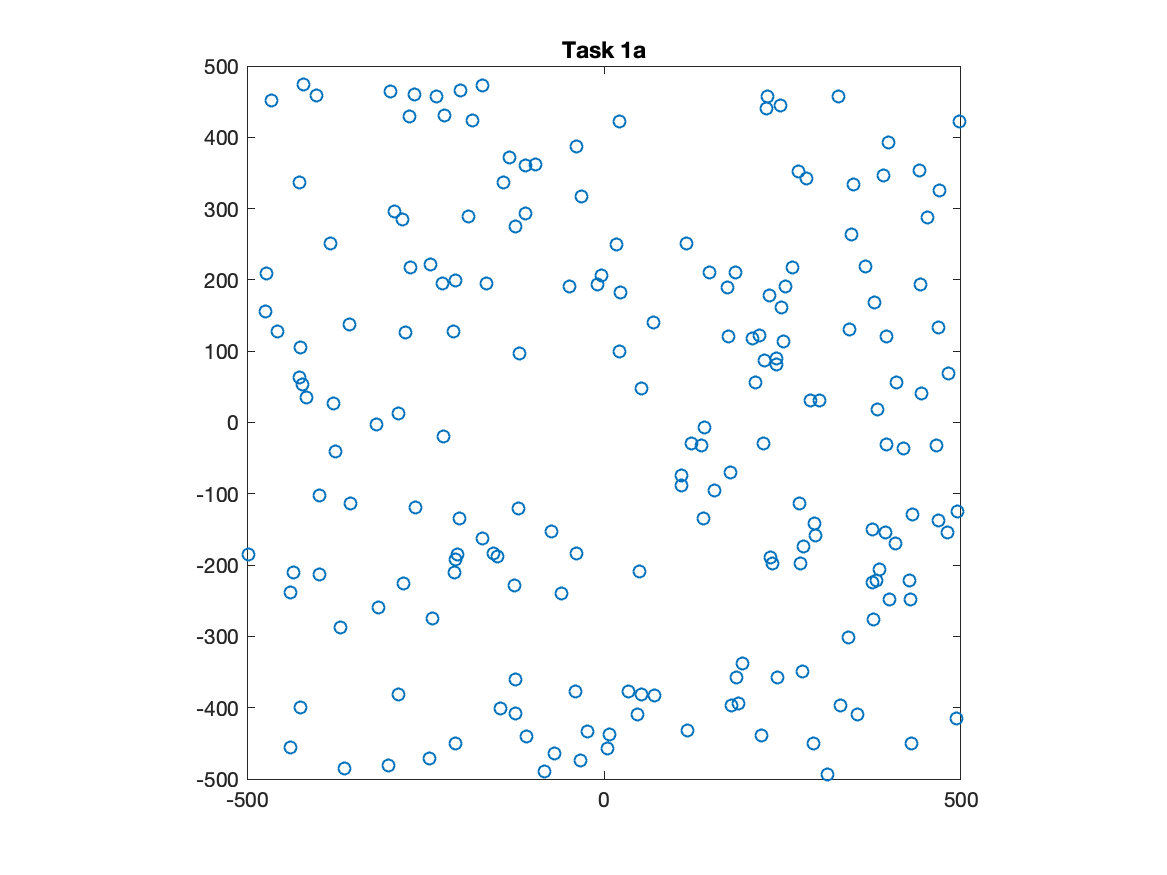
\includegraphics[width=\textwidth]{screenshot_taskb_10.png}
				\subcaption{Screenshot 10}
			\end{subfigure}
			\begin{subfigure}{0.25\textwidth}
				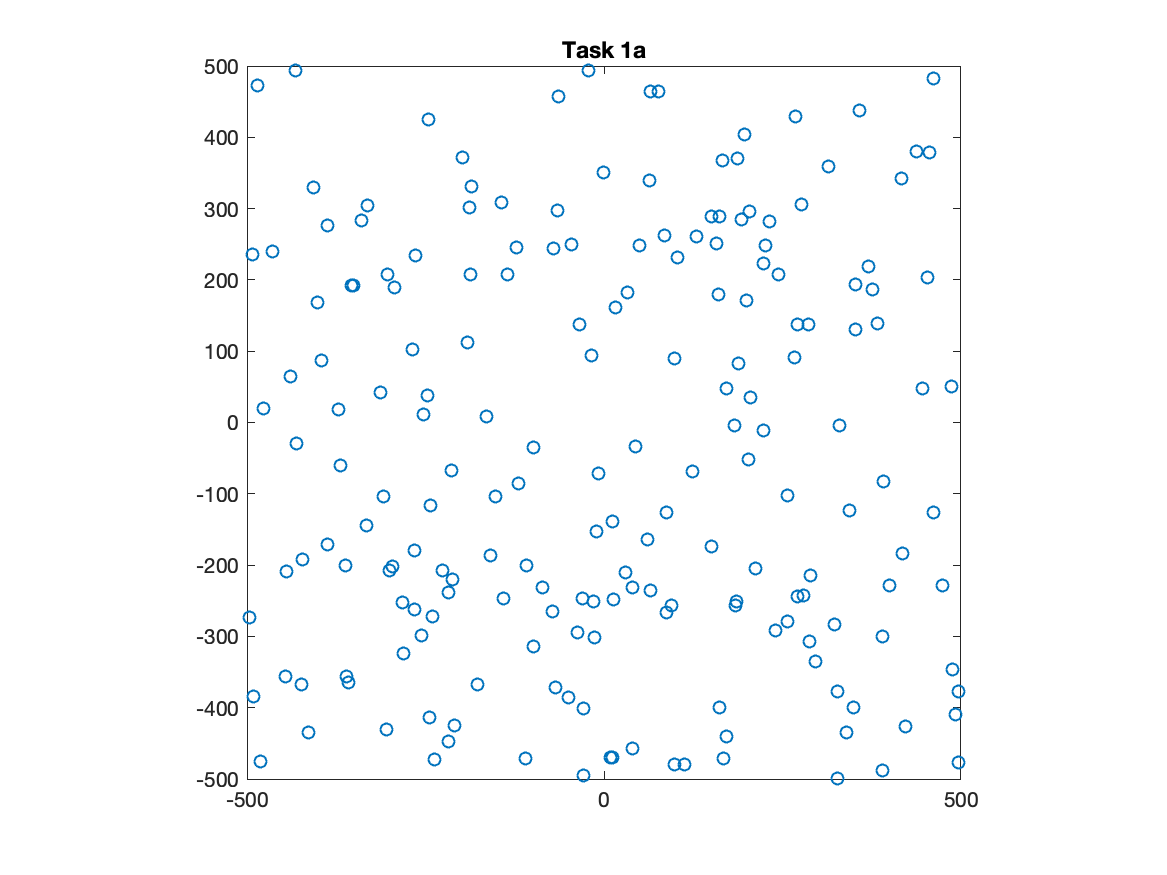
\includegraphics[width=\textwidth]{screenshot_taskb_15.png}
				\subcaption{Screenshot 15}
			\end{subfigure}
			\begin{subfigure}{0.25\textwidth}
				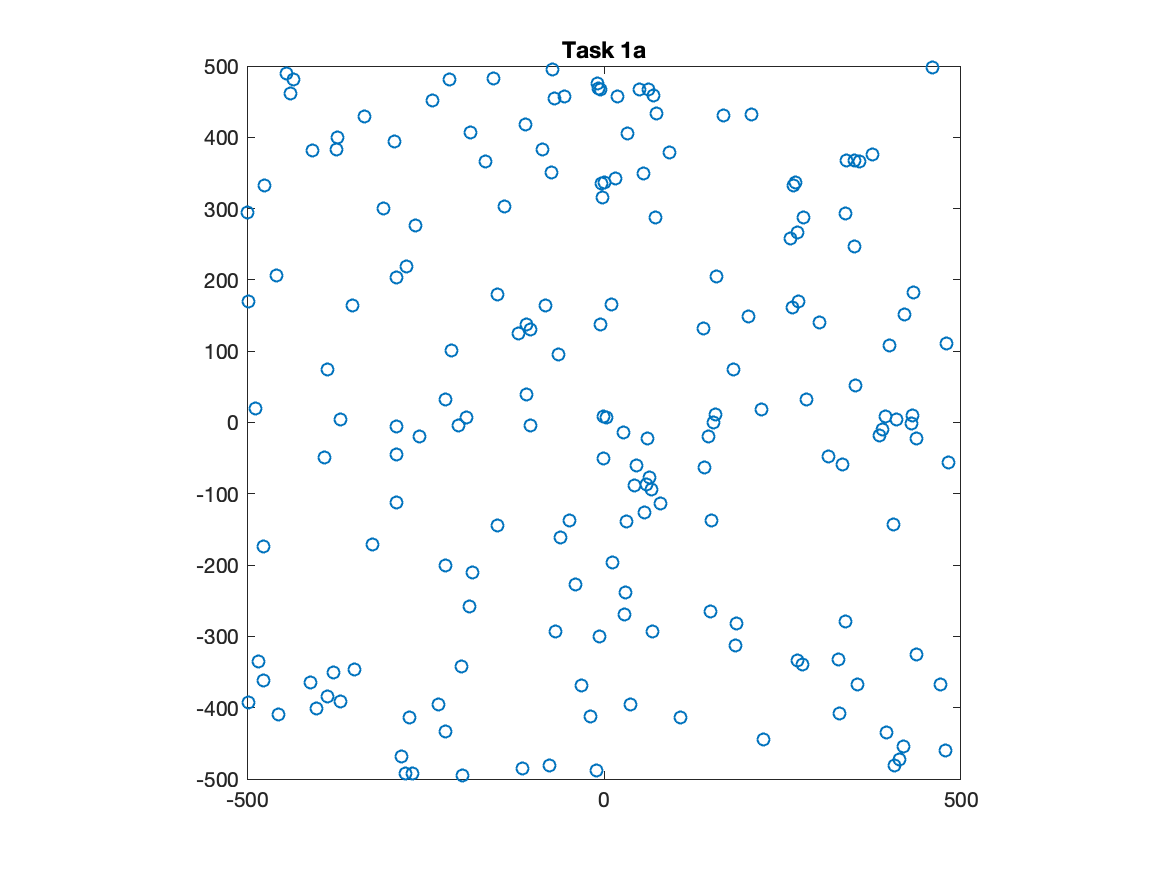
\includegraphics[width=\textwidth]{screenshot_taskb_25.png}
				\subcaption{Screenshot 25}
			\end{subfigure}
		\end{center}
		\caption{\label{fig_taskb_screenshots}\textit{Some of the screenshots from code ref.~\ref{code_taskb_screenshots}}}
	\end{figure}
	
	This code sends the particles off in a random direction at a random velocity, however it does not 'bounce' off the wall. In order to solve this, I used the \code{find} command (lines 32-35 in Appendix~\ref{apx_task1a}).	To take the screenshots required, I used modulo artithmetic take screenshots every time \code{t} is a multiple of 10. The code I used for is referenced~\ref{code_taskb_screenshots}. Some screenshots created by this are shown in figure~\ref{fig_taskb_screenshots}.
	
	\begin{equation} % Code to create the screenshots.
	\label{code_taskb_screenshots} 
	\begin{array}{ll}
	\code{if} & \code{mod(ta,10)==0  ta<=250}\\
	&\code{filename = ['screenshot\textunderscore taskb\textunderscore ' num2str(ta/10) '.png];}\\
	&\code{saveas(gcf,filename)}\\
	\code{end}&
	\end{array}
	\end{equation}

	\subsection{Task c) Adding a Trace behind Particles} 

	The first part is similar to Task 1a). I started off by changing: 
	\begin{itemize}
		\item any variable ending with \code{a} to \code{c} (i.e. \code{xa} $\Rightarrow$ \code{xc})
		\item the line \code{figure(1)} $\Rightarrow $ \code{figure(2)}
		\item the line \code{Na = randi([100 500],1,1);}  $\Rightarrow $ \code{Nc = randi([20 40],1,1);} (as only a few particles are needed).
		\item the time limit: the \code{while} loop is now until \code{t < = 100}.
		\item the number of screenshots: there is now only one when \code{tc == 99}
	\end{itemize}
	With the help of an M-file Alex shared (Pedcenko, 2018~\cite{MatlabTraceExample}), I added serveral features to my code, referenced~\ref{code_taskc_trace}. The output of this is shown in figure~\ref{fig_tracephoto}. 
	\begin{equation} % Code for the Trace of the particles
	\label{code_taskc_trace}
	\begin{array}{ll}
	\text{\textbf{With the previous variable definitions: }}	
	& \text{\textbf{Within the loop creating particle motion: }}\\
	\code{Xc = [xc];}		& \code{Xc = [Xc; xc];} \\
	\code{Yc = [yc];}		& \code{Yc = [Yc; yc];} \\ 
	\code{for i = 1:Nc}		& \code{hc.XData = xc;}\\
	\code{\ \ \ \ \ \ trc(i) = plot(Xc(:,i),Yc(:,i),'-k');}	&	\code{hc.YData = yc;}\\
	\code{end}&	\code{for i = 1:Nc}\\
	&\code{\ \ \ \ \ \ trc(i).XData=Xc(:,i);}\\
	&\code{\ \ \ \ \ \ trc(i).YData=Yc(:,i);}\\
	&  \code{end}
	\end{array}
	\end{equation}
	\begin{figure}[h!] % Output of the code for trace
		\begin{center}
		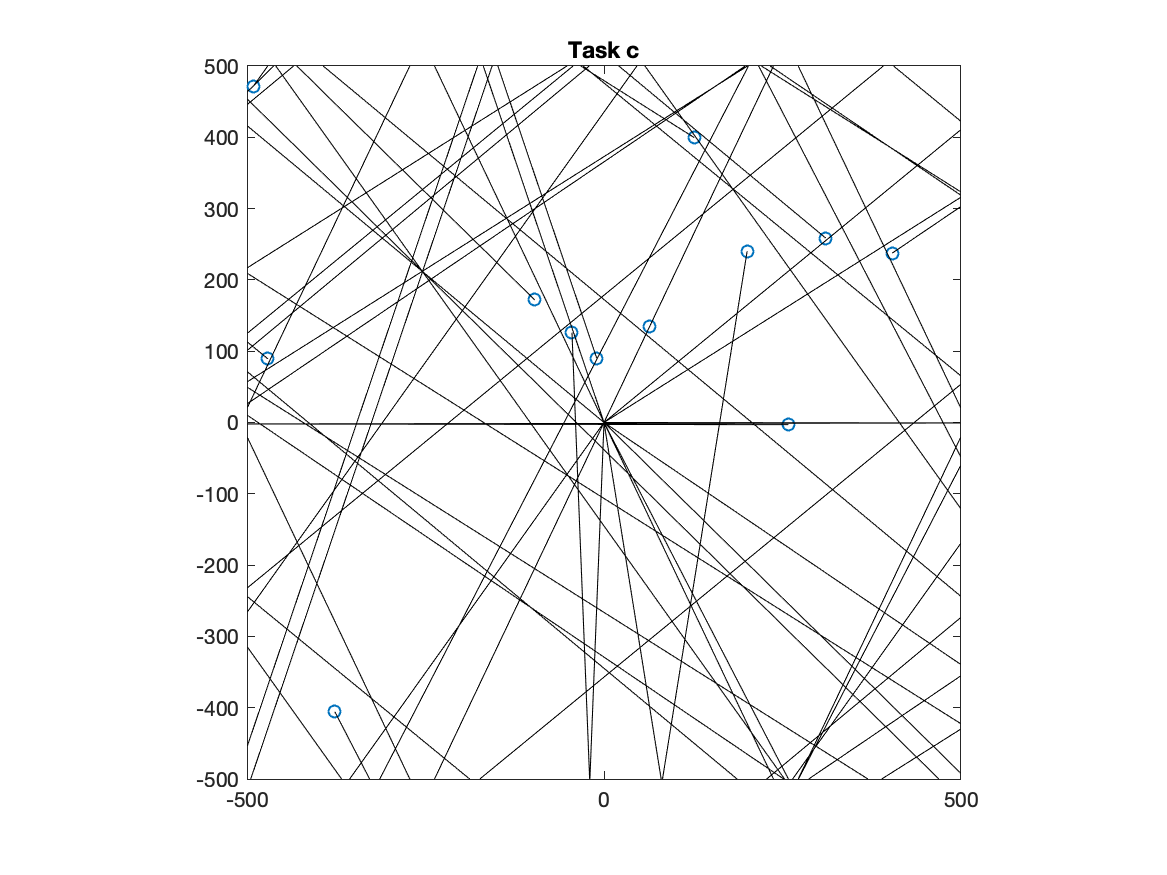
\includegraphics[width=0.35\textwidth]{screenshot_taskc.png}
		\caption{\textit{\label{fig_tracephoto}The figure resulting from the code ref.~\ref{code_taskc_trace}}}
		\end{center}
	\end{figure}
	
	\subsection{Task d) Action of Gravity} 
	
	Defining \code{g=9.8}, I added an updated calculation for \code{vyd}: $ v=v_0+gt $, by \code{vyd = vyd-g*dt}. The only major change from the previous code is shown in Appendix~\ref{apx_task1d}.
	
	\subsection{Task e) Loss of Energy on Collision}	
	For this task, I used a lot of the code from Task a). I added two variables to the ones in Table~\ref{tbl_variablestaska}, defined in Table~\ref{code_define_en}. When a particle hits the wall, its \code{en} value loses 10\%. Its velocity is then multipled by the new energy, so the particle slows down after each bounce. The code ref.~\ref{code_energydecrease} is used for this ($x$ values. For $y$ values, \code{x}$\Rightarrow$\code{y}). 
	\begin{table}[h!] % Variables added for task e
	\begin{tabular}{c|c|l}
	\textbf{Name} & \textbf{Job of Variable} & \textbf{Defined as}\\
	\hline\hline
	\code{En} & Array containing the energy of each individual particle & \code{= ones(Ne,1);}\\
	\code{Toten}& Plot of the time passed again the total energy in the system & \code{= plot(te,sum(en),'c+:');}
	\end{tabular}
	\caption{\label{code_define_en}Variables added to those in Tab.~\ref{tbl_variablestaska} for task 1e).}
	\end{table}
	
	\begin{equation}  % Energy decreases each bounce
	\label{code_energydecrease}
	\begin{array}{ll}
	\code{en(wallxe)}&\code{= 0.9 * en(wallxe);}\\
	\code{vxe(wallxe)}&\code{= vxe(wallxe)*-1.*en(wallxe);}
	\end{array}
	\end{equation}
	
	Some improvements I would make with this task include:
	\begin{itemize}
		\item making the particles move smoother in the figure,
		\item not having the particles leave the boundary at all, and
		\item starting the particles at random points in task d) instead of the origin.
	\end{itemize}
	
	
	\subsection{Task f) Plot of Total System Energy} % FINISH CODE & WRITE UP 
	
	To plot the sum of the energy of the particles from previous tasks, I added the variable \code{en$i$} ($i$ is the task), and then added a new figure to them. Prior to the motion creating while loop, I added the code referenced~\ref{code_energies}. In the while loop causing the particle motion, I added the second part of the code in Appendix~\ref{apx_task1e}. However, I didn't manage to get the line to stay. When I added similar code for tasks c) and d)\footnote{I removed the code from task c) because it interefered with figure~\ref{fig_tracephoto}}, I saw that in: 
	\begin{itemize}
		\item Tasks c) and d), the total energy is constant throughout.
		\item Task e), the total energy starts off constant, but begins decaying as soon as there are collisions. 
	\end{itemize}
	
	\begin{equation}
	\label{code_energies}
	\begin{array}{llrr}
	\code{figure($z$)} 					&&z \in \mathbb{R}\\
	\code{en$i$ = ones(N$i$,1)} 	&& i\text{ is the task}\\
	\code{toten$i$ = plot (t$i$,sum(en$i$),'c+:');}	&&\\
	\code{hold on}							&&\\
	\code{axis manual}						&&\\
	\code{axis([0 $u$ 0 (N$i$+5)])} && u\text{ is the time limit}
	\end{array}
	\end{equation}

	
	\subsection{Task g) Approach for Particle Motion with Collisions between Particles} % DO THIS
		
	If I were to create a code for this to happen, I would use the \code{find} function, similar to how I generated the 'bounce'. To show what I would do, I have used a pseudocode for MATLAB\textregistered, which is in appendix~\ref{apx_task1g}. 
	
	\section{Task 2: Symbolic Algebra} % Done.. Get figures in the right positions! 
	My cubic equation to complete the second task is:
	\begin{equation} % My cubic 
	\label{eq_cubic}
	y(x)=-3x^3+12x^2-9x-9
	\end{equation}
	To help with this task I used the Week 5 worksheet \cite{symbolicmath}. I had to firstly define $y(x)$. In order to do this, I used \code{syms x}, which introduces the symbolic variable $x$. I defined $y(x)$ by \code{y = -3 * x\^{}3 + 12 *  x\^{}2 - 9 * x - 9}.
	
	\subsection{Task a) Stationary Points of $y(x)$} % Done
	
	To find the stationary points, I differentiated, using the command \code{dy = diff(y)}. My new variable, \code{dy} is equal to $ \frac{d}{dx}\big[y(x)\big]=-9x^2+24x-9 $. To solve for when $\frac{dy}{dx}=0$, I used the code referenced~\ref{code_dy}. This gives the $x$ coordinates for the stationary points, as an array. In order to find the corresponding $y$ coordinates, I used the code referenced~\ref{code_ycoordinates}.
	
	\begin{equation} % Find x value of SP
	\label{code_dy} 
	\begin{array}{ll}
	\code{dy=diff y}& \\
	\code{format long}& \\
	\code{sp=double(solve(dy,0))}&
	\end{array}
	\end{equation}
	\begin{equation} % Sub in SP values of x into Y
	\label{code_ycoordinates}
	\begin{array}{ll}
	\code{pp1=double(subs(y,x,sp(1)))}& \\
	\code{pp2=double(subs(y,x,sp(2)))}& 
	\end{array}
	\end{equation}
	
	\begin{figure}[h!]
		\begin{subfigure}{0.5\textwidth}
			\label{fig_statpts}
			\begin{center}
				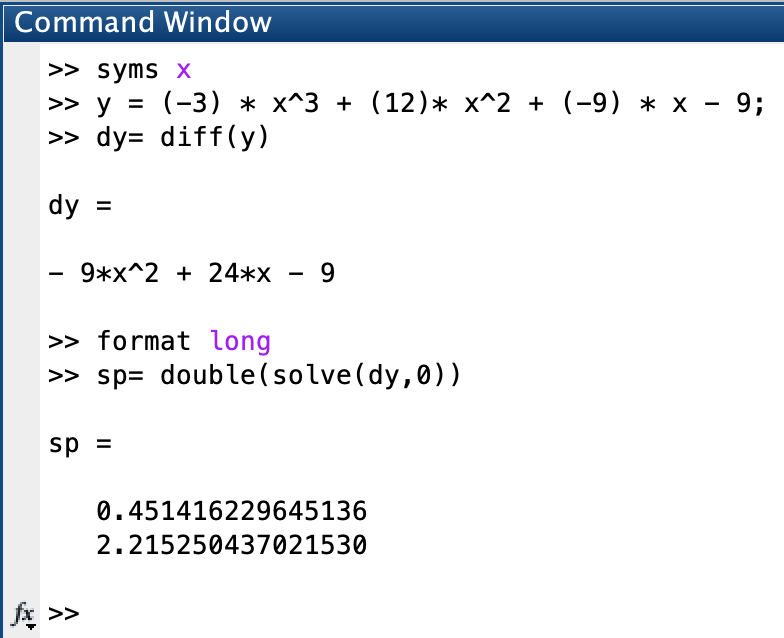
\includegraphics[width=0.55\textwidth]{a_screenshot.png}
			\end{center}
			\caption{\textit{Code Ref.~(\ref{code_dy})}}
		\end{subfigure}
		\begin{subfigure}{0.5\textwidth}
				\label{fig_statpts_yco}
				\begin{center}
					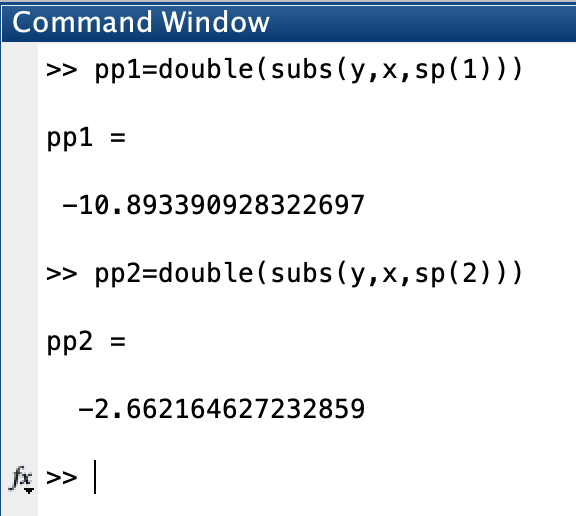
\includegraphics[width=0.5\textwidth]{a_screenshot2.png}
				\end{center}
				\caption{\textit{Code Ref.~(\ref{code_ycoordinates})}}
		\end{subfigure}
	\end{figure}

	\begin{flushleft}
	Once this was done, I used \code{pp = [pp1 pp2]}, to create an array with the $y$ co-ordinates of the stationary values in. The coordinates to my stationary points (to six significant figures) are:
	\end{flushleft}
	\begin{equation}
	\label{the_stationary_points}
	\begin{array}{rcl}
	(x_1,\ y_1) & = & (0.451416, -10.8934) \\
	(x_2,\ y_2) & = & (2.21525, -2.66216) 
	\end{array}
	\end{equation}

	\subsection{Task b) Second Derivatives of $y(x)$} % Done	
	
	\begin{equation}
	\label{code_secondder}
	\begin{array}{ll}
		\code{d2=diff dy;}& \\
		\code{cl=double(subs(d2,x,sp))}&
	\end{array}
	\end{equation}
	
	In order to assign the second derivitive test to the corresponding stationary point, I used the \code{find} function, which is between lines 7 and 11 in Appendix~\ref{apx_Task2}. From this code, we see that $(x_1, y_1)$ is a \textbf{local minima} and $(x_2, y_2)$ is a \textbf{local maxima}.
	
	\subsection{Task c) Plotting a Graph of a Function} % Done
	\label{section_2c}
	To plot $y(x)$, I used the \code{figure()} command to create a blank figure, on which $y(x)$ can be plotted. The full code for this is between lines 12 and 16 in Appendix~\ref{apx_Task2}. This will plot the cubic equation referenced~\ref{eq_cubic} between -1 and 4 in the $x$ direction and -12 and 0 in the $y$ direction. I chose this as both stationary points lie in this region. To add the markers if the maxima and minima (Ref.~\ref{the_stationary_points}) I used the code referenced~\ref{code:markers}, which, in the command window, gives figure~\ref{fig_plot2}.
	
	\begin{figure}[h!]
	\begin{subfigure}{0.5\textwidth}
		\begin{center}
			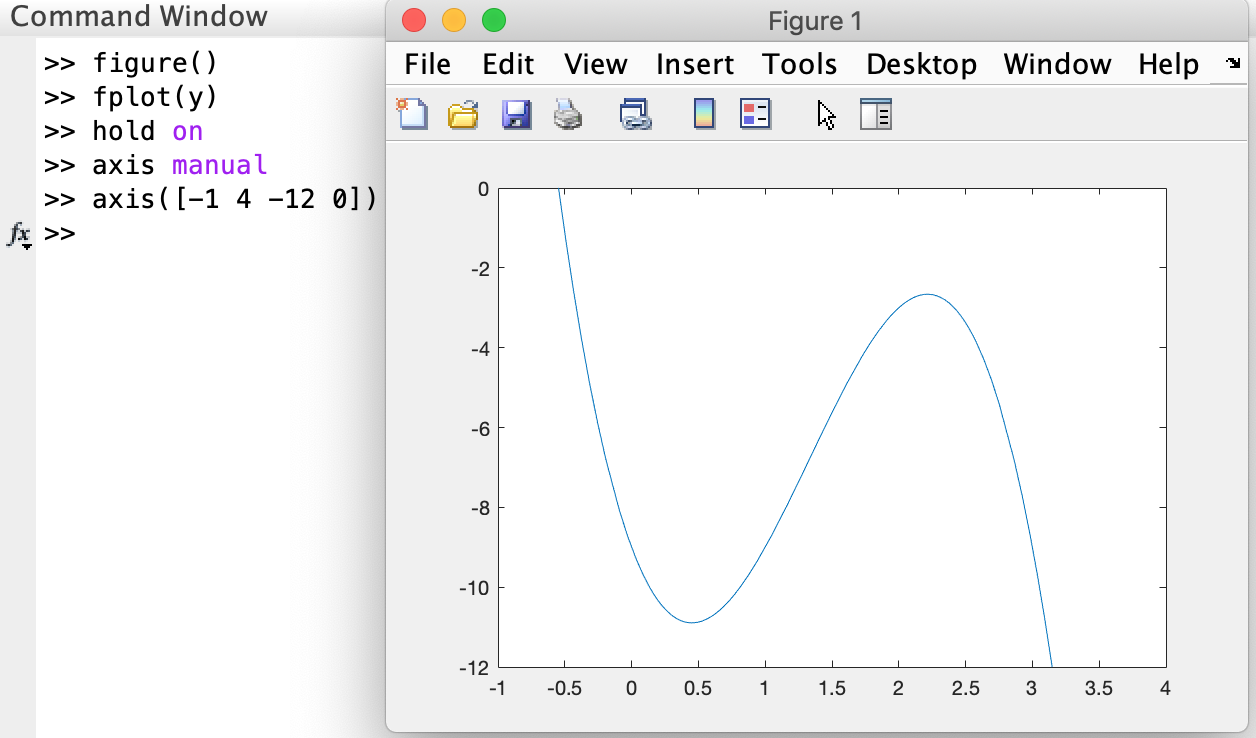
\includegraphics[width=0.85\textwidth]{c_screenshot.png}
		\end{center}
		\caption{\label{fig:plotofy}\textit{Plot of $y(x)$}}
	\end{subfigure}
	\begin{subfigure}{0.5\textwidth}
		\begin{center}
			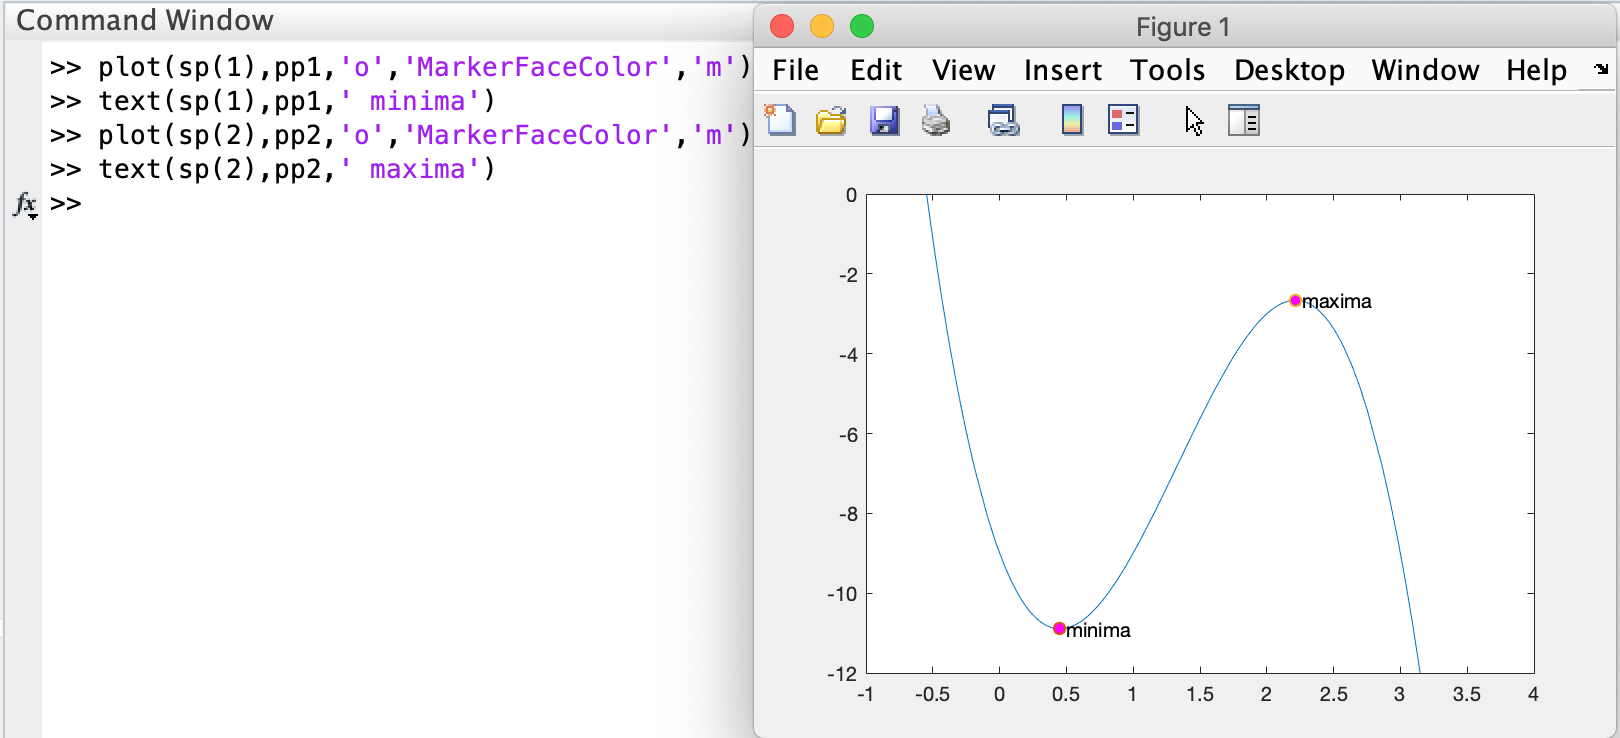
\includegraphics[width=0.95\textwidth]{c_screenshot2.png}
		\end{center}
		\caption{\textit{\label{fig_plot2}Plot of $y(x)$ with Labels}}
	\end{subfigure}
	\caption{Figures produced by code throughout Section~\ref{section_2c}}
	\end{figure}
	
	\begin{equation} % Code to make the markers
	\label{code:markers}
	\begin{array}{ll}
		\code{plot(sp(1),pp1,'o','MarkerFaceColor','m')}& \\
		\code{text(sp(1),pp1,' minima')} & \\
		\code{plot(sp(2),pp2,'o','MarkerFaceColor','m')} & \\
		\code{text(sp(2),pp2,' maxima')}
	\end{array}
	\end{equation}

	\subsection{Task d) Integration of $y(x)$} % Done // See about referencing

	$y(x)$ has one real root (Fig.~\ref{fig:plotofy}), so I integrated between the  real root and the first stationary point ($x_1,y_1$). I used  \code{root = double(solve(y==0))} to find the root, and  \code{integral = abs(double(int(y,root(1),sp(1)))} to integrate\footnote{\code{abs} ensures the inetgral is an absolute value--Area can not be negative.}. This gave figure~\ref{fig_complexroots}.

	\begin{figure}[h!]
		\begin{center}
			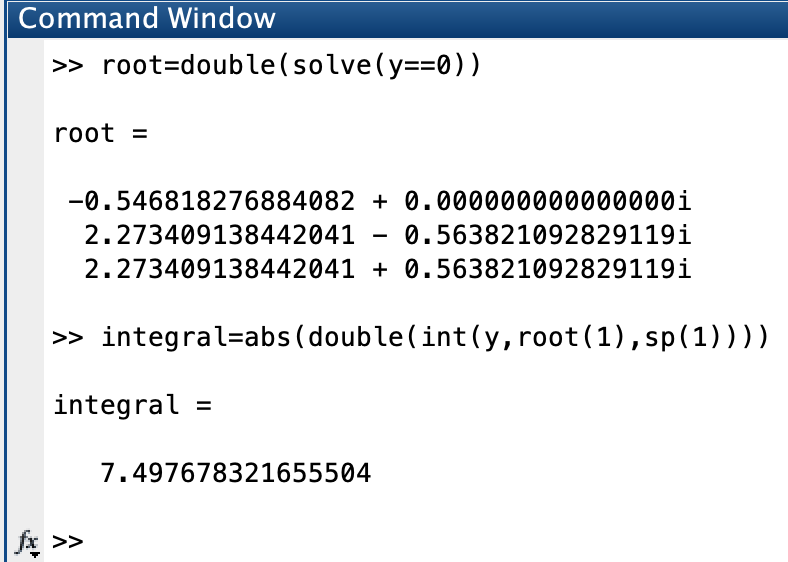
\includegraphics[width=0.35\textwidth]{d_screenshot.png}
		\end{center}
		\caption{\label{fig_complexroots}\textit{Integral of $y(x)$ between the $\mathbb{R}$ root and $(x_1,y_1)$}}
	\end{figure}
	We can see, if ${r}$ is the point where $y(x)=0,\ x\in\mathbb{R}$, and using $(x_1,y_1)$ (Ref.~(\ref{the_stationary_points}), then, to seven sig. fig.:
	$$ \int^{x_1}_{r} y(x)dx = 7.497678 $$ 
	
	\section{Conclusion}
	
	Prior to this semester, I had never used MATLAB\textregistered\ or \LaTeX before, and I am happy with how it has gone, however there are areas of improvement:
	\begin{itemize}
		\item The plot for task 1f) does not stay,
		\item The particles leave the boundaries for a split second, and so go out of the figure, and
		\item I didn't use any mathematical equations for energy, I just did a percentage.
	\end{itemize}
	
	
	\pagebreak
	\section{Appendices: Matlab Codes} % ADD FULL SECTIONS OF CODE HERE
			
	\subsection{Code for Task 1a) and 1b)}\label{apx_task1a}
	\lstinputlisting[language=Matlab, firstline=7, lastline=47]{task1code.m}
	
	\pagebreak
	
	\subsection{Code for Task 1c)}\label{apx_task1c}
	Replacing lines 7-20 in Section \ref{apx_task1a}:
	\lstinputlisting[language=Matlab, firstline=57,lastline=70]{task1code.m}
	\hrulefill
	
	After line 27-40 in Section \ref{apx_task1a}:
	\lstinputlisting[language=Matlab, firstline=85,lastline=98]{task1code.m}
	\hrulefill
	\subsection{Code for Task 1d)}\label{apx_task1d}
	Replacing lines 23 and 24 in Section \ref{apx_task1a}:
	\lstinputlisting[language=Matlab, firstline=131,lastline=132]{task1code.m}
	\pagebreak
	
	\subsection{Code for Task 1e) and 1f)}\label{apx_task1e}
	After line 21 in Section \ref{apx_task1a}:
	\lstinputlisting[language=Matlab, firstline=168,lastline=175]{task1code.m}
	
	\hrulefill
	
	Replacing all after line 29 in Section \ref{apx_task1a}:
	\lstinputlisting[language=Matlab, firstline=184,lastline=196]{task1code.m}
	
	\subsection{Pseudocode for Task 1g)}\label{apx_task1g}
	\lstinputlisting{task1dpseudocode.m}
	\pagebreak
	\subsection{Code for Task 2)}\label{apx_Task2}
	\lstinputlisting{task2code.m}

		
	\flushleft
	\thebibliography{9}
	
	\bibitem{MatlabHelp} MathWorks (2018){\it MATLAB\textregistered Documentation (Online Help)]} [online], avaliable from: $<$~ https://uk.mathworks.com/help/matlab/index.html~$>$ [5 December 2018]
	
	\bibitem{MatlabTraceExample} A Pedcenko (2018){\it An example of a project with the trace behind M-file} [online], available from: $<$~ https://cumoodle.coventry.ac.uk/pluginfile.php/2467358/mod{\textunderscore} resource/content/6/N{\textunderscore}projectiles.m~$>$ [7 December 2018]
	
	\bibitem{symbolicmath} {\it{Matlab PC Coursework for week 5}} [online], avaliable from: $<$~https://cumoodle.coventry.ac.uk/pluginfile.php/2451903/mod\textunderscore resource/content/2/Lab\%2005\%20Worksheet\%20--\%20Symbolic\%20Math.pdf~$>$
	
	
	
	\text{\textbf{\textit{Used to help compose the \LaTeX\ report:}}}
	
	\bibitem{Low07} R~Low (2007){\it \LaTeX: A cursory intoduction}, unpublished.
	\bibitem{Silveman07} JH~Silverman (2007){\it \AmS-\LaTeX\ Reference Card} [online], availiable from $<$http://www.math.brown.edu/~jhs/ReferenceCards/LaTeXRefCard.v2.0.pdf$>$ [11 December 2018]
	
	\endthebibliography

\end{document}